\documentclass[1p]{elsarticle_modified}
%\bibliographystyle{elsarticle-num}

%\usepackage[colorlinks]{hyperref}
%\usepackage{abbrmath_seonhwa} %\Abb, \Ascr, \Acal ,\Abf, \Afrak
\usepackage{amsfonts}
\usepackage{amssymb}
\usepackage{amsmath}
\usepackage{amsthm}
\usepackage{scalefnt}
\usepackage{amsbsy}
\usepackage{kotex}
\usepackage{caption}
\usepackage{subfig}
\usepackage{color}
\usepackage{graphicx}
\usepackage{xcolor} %% white, black, red, green, blue, cyan, magenta, yellow
\usepackage{float}
\usepackage{setspace}
\usepackage{hyperref}

\usepackage{tikz}
\usetikzlibrary{arrows}

\usepackage{multirow}
\usepackage{array} % fixed length table
\usepackage{hhline}

%%%%%%%%%%%%%%%%%%%%%
\makeatletter
\renewcommand*\env@matrix[1][\arraystretch]{%
	\edef\arraystretch{#1}%
	\hskip -\arraycolsep
	\let\@ifnextchar\new@ifnextchar
	\array{*\c@MaxMatrixCols c}}
\makeatother %https://tex.stackexchange.com/questions/14071/how-can-i-increase-the-line-spacing-in-a-matrix
%%%%%%%%%%%%%%%

\usepackage[normalem]{ulem}

\newcommand{\msout}[1]{\ifmmode\text{\sout{\ensuremath{#1}}}\else\sout{#1}\fi}
%SOURCE: \msout is \stkout macro in https://tex.stackexchange.com/questions/20609/strikeout-in-math-mode

\newcommand{\cancel}[1]{
	\ifmmode
	{\color{red}\msout{#1}}
	\else
	{\color{red}\sout{#1}}
	\fi
}

\newcommand{\add}[1]{
	{\color{blue}\uwave{#1}}
}

\newcommand{\replace}[2]{
	\ifmmode
	{\color{red}\msout{#1}}{\color{blue}\uwave{#2}}
	\else
	{\color{red}\sout{#1}}{\color{blue}\uwave{#2}}
	\fi
}

\newcommand{\Sol}{\mathcal{S}} %segment
\newcommand{\D}{D} %diagram
\newcommand{\A}{\mathcal{A}} %arc


%%%%%%%%%%%%%%%%%%%%%%%%%%%%%5 test

\def\sl{\operatorname{\textup{SL}}(2,\Cbb)}
\def\psl{\operatorname{\textup{PSL}}(2,\Cbb)}
\def\quan{\mkern 1mu \triangleright \mkern 1mu}

\theoremstyle{definition}
\newtheorem{thm}{Theorem}[section]
\newtheorem{prop}[thm]{Proposition}
\newtheorem{lem}[thm]{Lemma}
\newtheorem{ques}[thm]{Question}
\newtheorem{cor}[thm]{Corollary}
\newtheorem{defn}[thm]{Definition}
\newtheorem{exam}[thm]{Example}
\newtheorem{rmk}[thm]{Remark}
\newtheorem{alg}[thm]{Algorithm}

\newcommand{\I}{\sqrt{-1}}
\begin{document}

%\begin{frontmatter}
%
%\title{Boundary parabolic representations of knots up to 8 crossings}
%
%%% Group authors per affiliation:
%\author{Yunhi Cho} 
%\address{Department of Mathematics, University of Seoul, Seoul, Korea}
%\ead{yhcho@uos.ac.kr}
%
%
%\author{Seonhwa Kim} %\fnref{s_kim}}
%\address{Center for Geometry and Physics, Institute for Basic Science, Pohang, 37673, Korea}
%\ead{ryeona17@ibs.re.kr}
%
%\author{Hyuk Kim}
%\address{Department of Mathematical Sciences, Seoul National University, Seoul 08826, Korea}
%\ead{hyukkim@snu.ac.kr}
%
%\author{Seokbeom Yoon}
%\address{Department of Mathematical Sciences, Seoul National University, Seoul, 08826,  Korea}
%\ead{sbyoon15@snu.ac.kr}
%
%\begin{abstract}
%We find all boundary parabolic representation of knots up to 8 crossings.
%
%\end{abstract}
%\begin{keyword}
%    \MSC[2010] 57M25 
%\end{keyword}
%
%\end{frontmatter}

%\linenumbers
%\tableofcontents
%
\newcommand\colored[1]{\textcolor{white}{\rule[-0.35ex]{0.8em}{1.4ex}}\kern-0.8em\color{red} #1}%
%\newcommand\colored[1]{\textcolor{white}{ #1}\kern-2.17ex	\textcolor{white}{ #1}\kern-1.81ex	\textcolor{white}{ #1}\kern-2.15ex\color{red}#1	}

{\Large $\underline{12n_{0530}~(K12n_{0530})}$}

\setlength{\tabcolsep}{10pt}
\renewcommand{\arraystretch}{1.6}
\vspace{1cm}\begin{tabular}{m{100pt}>{\centering\arraybackslash}m{274pt}}
\multirow{5}{120pt}{
	\centering
	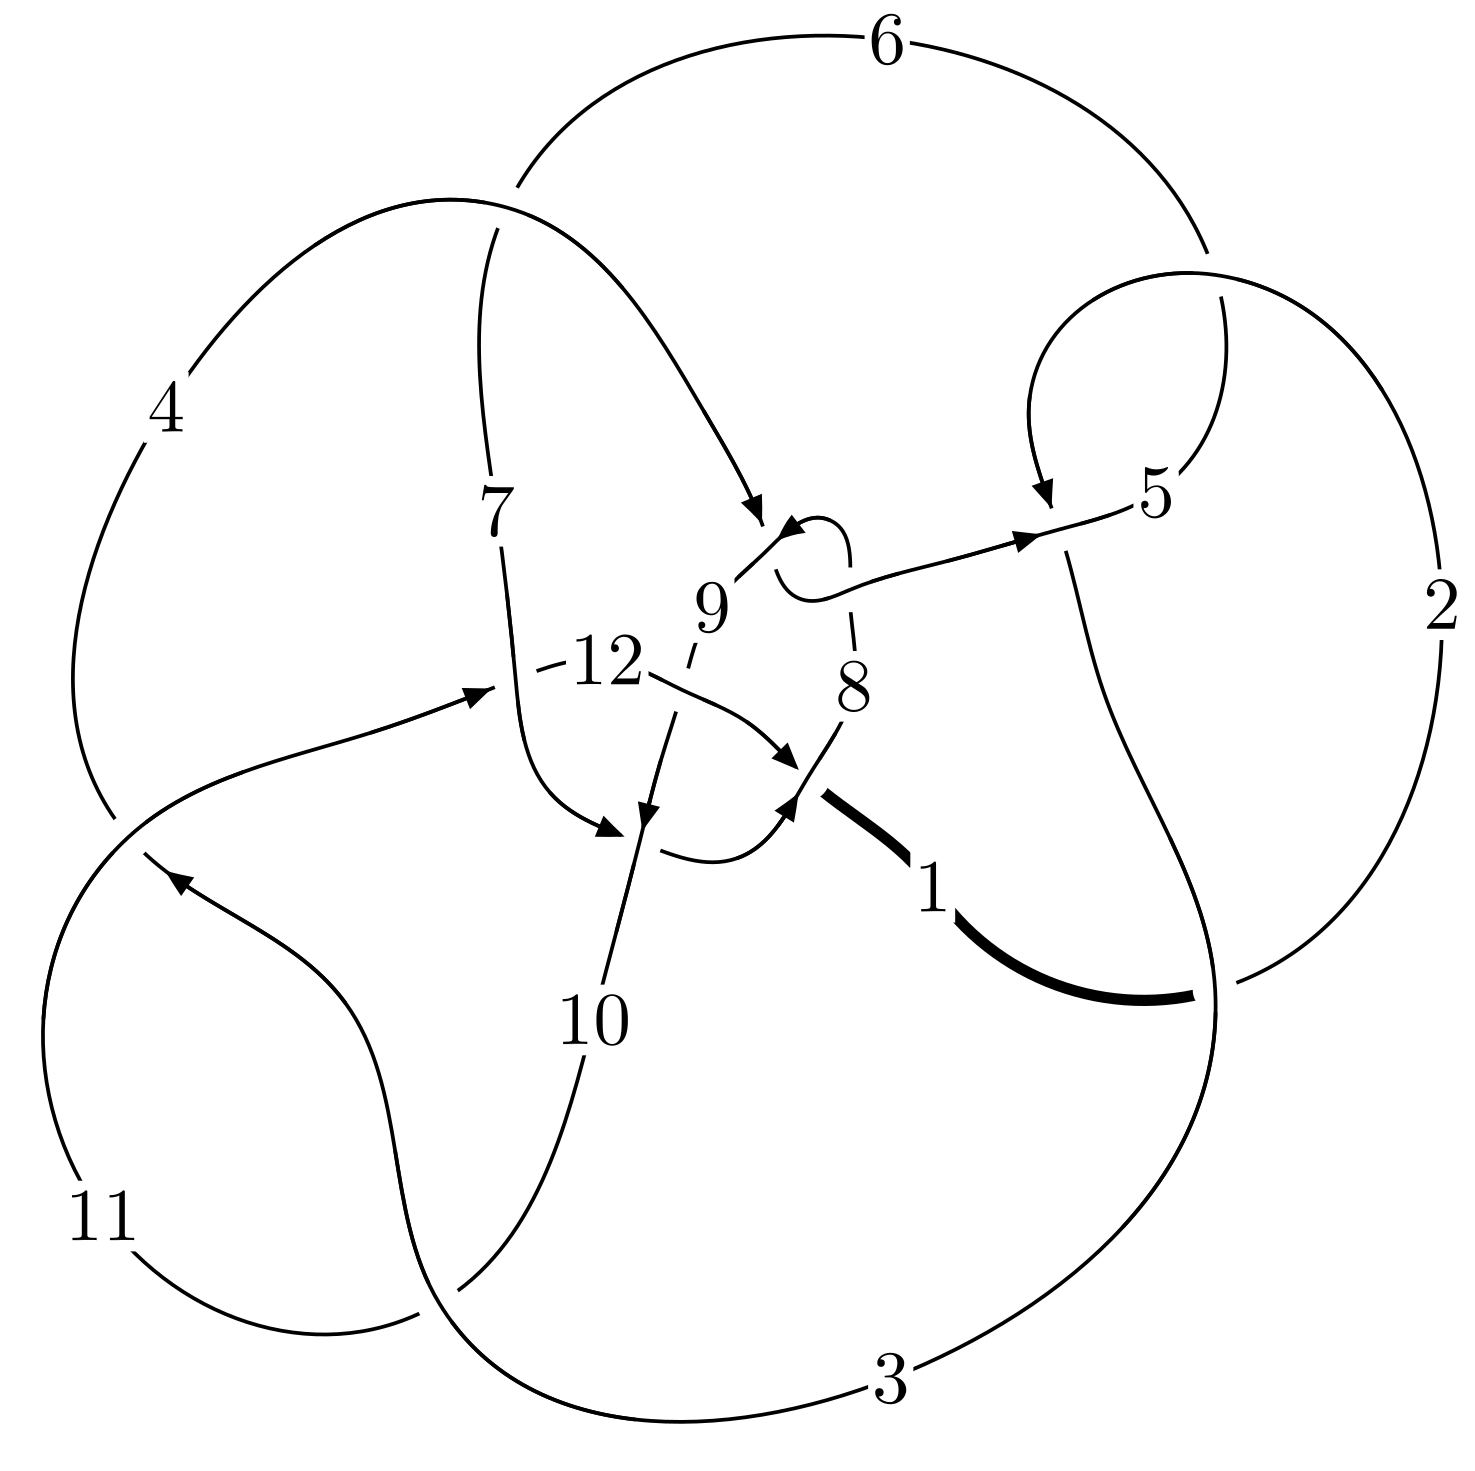
\includegraphics[width=112pt]{../../../GIT/diagram.site/Diagrams/png/2619_12n_0530.png}\\
\ \ \ A knot diagram\footnotemark}&
\allowdisplaybreaks
\textbf{Linearized knot diagam} \\
\cline{2-2}
 &
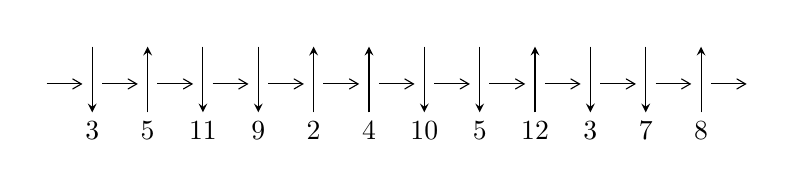
\begin{tikzpicture}[x=20pt, y=17pt]
	% nodes
	\node (C0) at (0, 0) {};
	\node (C1) at (1, 0) {};
	\node (C1U) at (1, +1) {};
	\node (C1D) at (1, -1) {3};

	\node (C2) at (2, 0) {};
	\node (C2U) at (2, +1) {};
	\node (C2D) at (2, -1) {5};

	\node (C3) at (3, 0) {};
	\node (C3U) at (3, +1) {};
	\node (C3D) at (3, -1) {11};

	\node (C4) at (4, 0) {};
	\node (C4U) at (4, +1) {};
	\node (C4D) at (4, -1) {9};

	\node (C5) at (5, 0) {};
	\node (C5U) at (5, +1) {};
	\node (C5D) at (5, -1) {2};

	\node (C6) at (6, 0) {};
	\node (C6U) at (6, +1) {};
	\node (C6D) at (6, -1) {4};

	\node (C7) at (7, 0) {};
	\node (C7U) at (7, +1) {};
	\node (C7D) at (7, -1) {10};

	\node (C8) at (8, 0) {};
	\node (C8U) at (8, +1) {};
	\node (C8D) at (8, -1) {5};

	\node (C9) at (9, 0) {};
	\node (C9U) at (9, +1) {};
	\node (C9D) at (9, -1) {12};

	\node (C10) at (10, 0) {};
	\node (C10U) at (10, +1) {};
	\node (C10D) at (10, -1) {3};

	\node (C11) at (11, 0) {};
	\node (C11U) at (11, +1) {};
	\node (C11D) at (11, -1) {7};

	\node (C12) at (12, 0) {};
	\node (C12U) at (12, +1) {};
	\node (C12D) at (12, -1) {8};
	\node (C13) at (13, 0) {};

	% arrows
	\draw[->,>={angle 60}]
	(C0) edge (C1) (C1) edge (C2) (C2) edge (C3) (C3) edge (C4) (C4) edge (C5) (C5) edge (C6) (C6) edge (C7) (C7) edge (C8) (C8) edge (C9) (C9) edge (C10) (C10) edge (C11) (C11) edge (C12) (C12) edge (C13) ;	\draw[->,>=stealth]
	(C1U) edge (C1D) (C2D) edge (C2U) (C3U) edge (C3D) (C4U) edge (C4D) (C5D) edge (C5U) (C6D) edge (C6U) (C7U) edge (C7D) (C8U) edge (C8D) (C9D) edge (C9U) (C10U) edge (C10D) (C11U) edge (C11D) (C12D) edge (C12U) ;
	\end{tikzpicture} \\
\hhline{~~} \\& 
\textbf{Solving Sequence} \\ \cline{2-2} 
 &
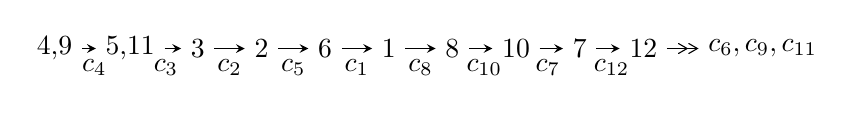
\begin{tikzpicture}[x=23pt, y=7pt]
	% node
	\node (A0) at (-1/8, 0) {4,9};
	\node (A1) at (17/16, 0) {5,11};
	\node (A2) at (17/8, 0) {3};
	\node (A3) at (25/8, 0) {2};
	\node (A4) at (33/8, 0) {6};
	\node (A5) at (41/8, 0) {1};
	\node (A6) at (49/8, 0) {8};
	\node (A7) at (57/8, 0) {10};
	\node (A8) at (65/8, 0) {7};
	\node (A9) at (73/8, 0) {12};
	\node (C1) at (1/2, -1) {$c_{4}$};
	\node (C2) at (13/8, -1) {$c_{3}$};
	\node (C3) at (21/8, -1) {$c_{2}$};
	\node (C4) at (29/8, -1) {$c_{5}$};
	\node (C5) at (37/8, -1) {$c_{1}$};
	\node (C6) at (45/8, -1) {$c_{8}$};
	\node (C7) at (53/8, -1) {$c_{10}$};
	\node (C8) at (61/8, -1) {$c_{7}$};
	\node (C9) at (69/8, -1) {$c_{12}$};
	\node (A10) at (11, 0) {$c_{6},c_{9},c_{11}$};

	% edge
	\draw[->,>=stealth]	
	(A0) edge (A1) (A1) edge (A2) (A2) edge (A3) (A3) edge (A4) (A4) edge (A5) (A5) edge (A6) (A6) edge (A7) (A7) edge (A8) (A8) edge (A9) ;
	\draw[->>,>={angle 60}]	
	(A9) edge (A10);
\end{tikzpicture} \\ 

\end{tabular} \\

\footnotetext{
The image of knot diagram is generated by the software ``\textbf{Draw programme}" developed by Andrew Bartholomew(\url{http://www.layer8.co.uk/maths/draw/index.htm\#Running-draw}), where we modified some parts for our purpose(\url{https://github.com/CATsTAILs/LinksPainter}).
}\phantom \\ \newline 
\centering \textbf{Ideals for irreducible components\footnotemark of $X_{\text{par}}$} 
 
\begin{align*}
I^u_{1}&=\langle 
-3.64573\times10^{258} u^{71}+1.93369\times10^{258} u^{70}+\cdots+2.61570\times10^{260} b-8.84362\times10^{260},\\
\phantom{I^u_{1}}&\phantom{= \langle  }1.94505\times10^{261} u^{71}-9.37390\times10^{260} u^{70}+\cdots+1.85715\times10^{262} a+2.78533\times10^{263},\\
\phantom{I^u_{1}}&\phantom{= \langle  }u^{72}+7 u^{70}+\cdots+174 u+71\rangle \\
I^u_{2}&=\langle 
2184459735 u^{30}+2467043153 u^{29}+\cdots+148046503 b+1530935116,\\
\phantom{I^u_{2}}&\phantom{= \langle  }-5788205505 u^{30}-2520329514 u^{29}+\cdots+148046503 a-9787930487,\;u^{31}+u^{30}+\cdots+u-1\rangle \\
\\
\end{align*}
\raggedright * 2 irreducible components of $\dim_{\mathbb{C}}=0$, with total 103 representations.\\
\footnotetext{All coefficients of polynomials are rational numbers. But the coefficients are sometimes approximated in decimal forms when there is not enough margin.}
\newpage
\renewcommand{\arraystretch}{1}
\centering \section*{I. $I^u_{1}= \langle -3.65\times10^{258} u^{71}+1.93\times10^{258} u^{70}+\cdots+2.62\times10^{260} b-8.84\times10^{260},\;1.95\times10^{261} u^{71}-9.37\times10^{260} u^{70}+\cdots+1.86\times10^{262} a+2.79\times10^{263},\;u^{72}+7 u^{70}+\cdots+174 u+71 \rangle$}
\flushleft \textbf{(i) Arc colorings}\\
\begin{tabular}{m{7pt} m{180pt} m{7pt} m{180pt} }
\flushright $a_{4}=$&$\begin{pmatrix}1\\0\end{pmatrix}$ \\
\flushright $a_{9}=$&$\begin{pmatrix}0\\u\end{pmatrix}$ \\
\flushright $a_{5}=$&$\begin{pmatrix}1\\u^2\end{pmatrix}$ \\
\flushright $a_{11}=$&$\begin{pmatrix}-0.104733 u^{71}+0.0504747 u^{70}+\cdots-10.2744 u-14.9979\\0.0139379 u^{71}-0.00739262 u^{70}+\cdots+0.899364 u+3.38097\end{pmatrix}$ \\
\flushright $a_{3}=$&$\begin{pmatrix}-0.100244 u^{71}+0.0145687 u^{70}+\cdots-6.20768 u-21.3805\\0.0524115 u^{71}-0.0459288 u^{70}+\cdots+11.4091 u+1.78594\end{pmatrix}$ \\
\flushright $a_{2}=$&$\begin{pmatrix}-0.127174 u^{71}+0.0337253 u^{70}+\cdots-13.0344 u-24.2008\\0.0395871 u^{71}-0.0395261 u^{70}+\cdots+9.98786 u+0.425816\end{pmatrix}$ \\
\flushright $a_{6}=$&$\begin{pmatrix}0.156586 u^{71}-0.111459 u^{70}+\cdots+35.4012 u+9.44122\\0.104480 u^{71}-0.0235722 u^{70}+\cdots+11.3081 u+19.1362\end{pmatrix}$ \\
\flushright $a_{1}=$&$\begin{pmatrix}-0.163406 u^{71}+0.0989962 u^{70}+\cdots-20.5083 u-13.3356\\-0.252000 u^{71}+0.111375 u^{70}+\cdots-34.9609 u-28.5427\end{pmatrix}$ \\
\flushright $a_{8}=$&$\begin{pmatrix}u\\u^3+u\end{pmatrix}$ \\
\flushright $a_{10}=$&$\begin{pmatrix}0.0257924 u^{71}+0.00721650 u^{70}+\cdots-4.53635 u+7.33620\\0.101128 u^{71}-0.0222456 u^{70}+\cdots+15.6108 u+16.7202\end{pmatrix}$ \\
\flushright $a_{7}=$&$\begin{pmatrix}0.261066 u^{71}-0.135031 u^{70}+\cdots+46.7093 u+28.5775\\0.104480 u^{71}-0.0235722 u^{70}+\cdots+11.3081 u+19.1362\end{pmatrix}$ \\
\flushright $a_{12}=$&$\begin{pmatrix}-0.173734 u^{71}+0.110746 u^{70}+\cdots-23.3198 u-13.1488\\-0.269089 u^{71}+0.124908 u^{70}+\cdots-39.0835 u-29.1901\end{pmatrix}$\\&\end{tabular}
\flushleft \textbf{(ii) Obstruction class $= -1$}\\~\\
\flushleft \textbf{(iii) Cusp Shapes $= -0.631363 u^{71}+0.329602 u^{70}+\cdots-114.221 u-62.1901$}\\~\\
\newpage\renewcommand{\arraystretch}{1}
\flushleft \textbf{(iv) u-Polynomials at the component}\newline \\
\begin{tabular}{m{50pt}|m{274pt}}
Crossings & \hspace{64pt}u-Polynomials at each crossing \\
\hline $$\begin{aligned}c_{1}\end{aligned}$$&$\begin{aligned}
&u^{72}+90 u^{71}+\cdots+1404496977 u+27447121
\end{aligned}$\\
\hline $$\begin{aligned}c_{2},c_{5}\end{aligned}$$&$\begin{aligned}
&u^{72}+4 u^{71}+\cdots-28717 u+5239
\end{aligned}$\\
\hline $$\begin{aligned}c_{3},c_{10}\end{aligned}$$&$\begin{aligned}
&u^{72}+2 u^{71}+\cdots+1164 u+89
\end{aligned}$\\
\hline $$\begin{aligned}c_{4},c_{8}\end{aligned}$$&$\begin{aligned}
&u^{72}+7 u^{70}+\cdots-174 u+71
\end{aligned}$\\
\hline $$\begin{aligned}c_{6}\end{aligned}$$&$\begin{aligned}
&u^{72}+12 u^{71}+\cdots+183732 u+262579
\end{aligned}$\\
\hline $$\begin{aligned}c_{7}\end{aligned}$$&$\begin{aligned}
&u^{72}-11 u^{70}+\cdots-251726 u+58649
\end{aligned}$\\
\hline $$\begin{aligned}c_{9}\end{aligned}$$&$\begin{aligned}
&u^{72}+3 u^{71}+\cdots+92 u+29
\end{aligned}$\\
\hline $$\begin{aligned}c_{11}\end{aligned}$$&$\begin{aligned}
&u^{72}+u^{71}+\cdots-2131 u+145
\end{aligned}$\\
\hline $$\begin{aligned}c_{12}\end{aligned}$$&$\begin{aligned}
&u^{72}- u^{71}+\cdots+9071598635 u+6503913561
\end{aligned}$\\
\hline
\end{tabular}\\~\\
\newpage\renewcommand{\arraystretch}{1}
\flushleft \textbf{(v) Riley Polynomials at the component}\newline \\
\begin{tabular}{m{50pt}|m{274pt}}
Crossings & \hspace{64pt}Riley Polynomials at each crossing \\
\hline $$\begin{aligned}c_{1}\end{aligned}$$&$\begin{aligned}
&y^{72}-202 y^{71}+\cdots+499387466684415153 y+753344451188641
\end{aligned}$\\
\hline $$\begin{aligned}c_{2},c_{5}\end{aligned}$$&$\begin{aligned}
&y^{72}+90 y^{71}+\cdots+1404496977 y+27447121
\end{aligned}$\\
\hline $$\begin{aligned}c_{3},c_{10}\end{aligned}$$&$\begin{aligned}
&y^{72}-56 y^{71}+\cdots-188640 y+7921
\end{aligned}$\\
\hline $$\begin{aligned}c_{4},c_{8}\end{aligned}$$&$\begin{aligned}
&y^{72}+14 y^{71}+\cdots-52712 y+5041
\end{aligned}$\\
\hline $$\begin{aligned}c_{6}\end{aligned}$$&$\begin{aligned}
&y^{72}+70 y^{71}+\cdots+2835486348132 y+68947731241
\end{aligned}$\\
\hline $$\begin{aligned}c_{7}\end{aligned}$$&$\begin{aligned}
&y^{72}-22 y^{71}+\cdots-71347990678 y+3439705201
\end{aligned}$\\
\hline $$\begin{aligned}c_{9}\end{aligned}$$&$\begin{aligned}
&y^{72}+9 y^{71}+\cdots+38110 y+841
\end{aligned}$\\
\hline $$\begin{aligned}c_{11}\end{aligned}$$&$\begin{aligned}
&y^{72}-13 y^{71}+\cdots-1039701 y+21025
\end{aligned}$\\
\hline $$\begin{aligned}c_{12}\end{aligned}$$&$\begin{aligned}
&y^{72}+77 y^{71}+\cdots+3.46\times10^{20} y+4.23\times10^{19}
\end{aligned}$\\
\hline
\end{tabular}\\~\\
\newpage\flushleft \textbf{(vi) Complex Volumes and Cusp Shapes}
$$\begin{array}{c|c|c}  
\text{Solutions to }I^u_{1}& \I (\text{vol} + \sqrt{-1}CS) & \text{Cusp shape}\\
 \hline 
\begin{aligned}
u &= \phantom{-}0.395735 + 0.962899 I \\
a &= \phantom{-}0.15710 - 1.90724 I \\
b &= \phantom{-}1.103020 + 0.378441 I\end{aligned}
 & -2.35206 - 4.90102 I & \phantom{-0.000000 } 0 \\ \hline\begin{aligned}
u &= \phantom{-}0.395735 - 0.962899 I \\
a &= \phantom{-}0.15710 + 1.90724 I \\
b &= \phantom{-}1.103020 - 0.378441 I\end{aligned}
 & -2.35206 + 4.90102 I & \phantom{-0.000000 } 0 \\ \hline\begin{aligned}
u &= \phantom{-}0.449062 + 0.795024 I \\
a &= -0.122453 - 0.304927 I \\
b &= -0.087555 + 0.465957 I\end{aligned}
 & \phantom{-}0.05590 - 1.89763 I & -1.60993 + 3.15256 I \\ \hline\begin{aligned}
u &= \phantom{-}0.449062 - 0.795024 I \\
a &= -0.122453 + 0.304927 I \\
b &= -0.087555 - 0.465957 I\end{aligned}
 & \phantom{-}0.05590 + 1.89763 I & -1.60993 - 3.15256 I \\ \hline\begin{aligned}
u &= \phantom{-}0.121973 + 1.102890 I \\
a &= -0.886065 - 0.527000 I \\
b &= -0.440152 + 0.475467 I\end{aligned}
 & \phantom{-}3.69129 - 1.79239 I & \phantom{-0.000000 } 0 \\ \hline\begin{aligned}
u &= \phantom{-}0.121973 - 1.102890 I \\
a &= -0.886065 + 0.527000 I \\
b &= -0.440152 - 0.475467 I\end{aligned}
 & \phantom{-}3.69129 + 1.79239 I & \phantom{-0.000000 } 0 \\ \hline\begin{aligned}
u &= \phantom{-}0.051307 + 0.865237 I \\
a &= -1.073040 - 0.163089 I \\
b &= \phantom{-}0.964573 + 0.239283 I\end{aligned}
 & -0.715343 - 0.560826 I & -2.22835 + 1.84045 I \\ \hline\begin{aligned}
u &= \phantom{-}0.051307 - 0.865237 I \\
a &= -1.073040 + 0.163089 I \\
b &= \phantom{-}0.964573 - 0.239283 I\end{aligned}
 & -0.715343 + 0.560826 I & -2.22835 - 1.84045 I \\ \hline\begin{aligned}
u &= \phantom{-}0.854276 + 0.144443 I \\
a &= \phantom{-}1.394460 + 0.022960 I \\
b &= \phantom{-}1.52014 - 0.19291 I\end{aligned}
 & -5.10447 + 1.24571 I & -11.85389 - 4.33977 I \\ \hline\begin{aligned}
u &= \phantom{-}0.854276 - 0.144443 I \\
a &= \phantom{-}1.394460 - 0.022960 I \\
b &= \phantom{-}1.52014 + 0.19291 I\end{aligned}
 & -5.10447 - 1.24571 I & -11.85389 + 4.33977 I\\
 \hline 
 \end{array}$$\newpage$$\begin{array}{c|c|c}  
\text{Solutions to }I^u_{1}& \I (\text{vol} + \sqrt{-1}CS) & \text{Cusp shape}\\
 \hline 
\begin{aligned}
u &= \phantom{-}0.540643 + 1.035120 I \\
a &= -1.01016 + 1.22898 I \\
b &= -1.026380 - 0.257760 I\end{aligned}
 & -2.36515 - 4.35350 I & \phantom{-0.000000 } 0 \\ \hline\begin{aligned}
u &= \phantom{-}0.540643 - 1.035120 I \\
a &= -1.01016 - 1.22898 I \\
b &= -1.026380 + 0.257760 I\end{aligned}
 & -2.36515 + 4.35350 I & \phantom{-0.000000 } 0 \\ \hline\begin{aligned}
u &= -0.836968 + 0.820484 I \\
a &= \phantom{-}0.062748 + 0.354211 I \\
b &= -0.028412 + 0.257770 I\end{aligned}
 & -7.21762 + 1.57842 I & \phantom{-0.000000 } 0 \\ \hline\begin{aligned}
u &= -0.836968 - 0.820484 I \\
a &= \phantom{-}0.062748 - 0.354211 I \\
b &= -0.028412 - 0.257770 I\end{aligned}
 & -7.21762 - 1.57842 I & \phantom{-0.000000 } 0 \\ \hline\begin{aligned}
u &= -0.089104 + 1.169450 I \\
a &= \phantom{-}1.390420 + 0.100465 I \\
b &= \phantom{-}0.418314 - 0.347525 I\end{aligned}
 & \phantom{-}2.56389 + 4.98234 I & \phantom{-0.000000 } 0 \\ \hline\begin{aligned}
u &= -0.089104 - 1.169450 I \\
a &= \phantom{-}1.390420 - 0.100465 I \\
b &= \phantom{-}0.418314 + 0.347525 I\end{aligned}
 & \phantom{-}2.56389 - 4.98234 I & \phantom{-0.000000 } 0 \\ \hline\begin{aligned}
u &= \phantom{-}1.146330 + 0.264545 I \\
a &= -1.42952 + 0.07044 I \\
b &= -1.293780 + 0.058915 I\end{aligned}
 & -5.24347 - 1.12672 I & \phantom{-0.000000 } 0 \\ \hline\begin{aligned}
u &= \phantom{-}1.146330 - 0.264545 I \\
a &= -1.42952 - 0.07044 I \\
b &= -1.293780 - 0.058915 I\end{aligned}
 & -5.24347 + 1.12672 I & \phantom{-0.000000 } 0 \\ \hline\begin{aligned}
u &= \phantom{-}0.443052 + 0.675051 I \\
a &= -0.782382 + 0.844362 I \\
b &= \phantom{-}0.437835 - 0.368886 I\end{aligned}
 & -0.38463 - 1.62177 I & -3.30795 + 2.54804 I \\ \hline\begin{aligned}
u &= \phantom{-}0.443052 - 0.675051 I \\
a &= -0.782382 - 0.844362 I \\
b &= \phantom{-}0.437835 + 0.368886 I\end{aligned}
 & -0.38463 + 1.62177 I & -3.30795 - 2.54804 I\\
 \hline 
 \end{array}$$\newpage$$\begin{array}{c|c|c}  
\text{Solutions to }I^u_{1}& \I (\text{vol} + \sqrt{-1}CS) & \text{Cusp shape}\\
 \hline 
\begin{aligned}
u &= -0.967859 + 0.698281 I \\
a &= -1.55826 - 0.52021 I \\
b &= -1.54355 + 0.43095 I\end{aligned}
 & -5.51623 + 9.76846 I & \phantom{-0.000000 } 0 \\ \hline\begin{aligned}
u &= -0.967859 - 0.698281 I \\
a &= -1.55826 + 0.52021 I \\
b &= -1.54355 - 0.43095 I\end{aligned}
 & -5.51623 - 9.76846 I & \phantom{-0.000000 } 0 \\ \hline\begin{aligned}
u &= -1.029520 + 0.617322 I \\
a &= \phantom{-}1.55254 + 0.54349 I \\
b &= \phantom{-}1.48143 - 0.48596 I\end{aligned}
 & -5.12009 + 3.07867 I & \phantom{-0.000000 } 0 \\ \hline\begin{aligned}
u &= -1.029520 - 0.617322 I \\
a &= \phantom{-}1.55254 - 0.54349 I \\
b &= \phantom{-}1.48143 + 0.48596 I\end{aligned}
 & -5.12009 - 3.07867 I & \phantom{-0.000000 } 0 \\ \hline\begin{aligned}
u &= -0.303232 + 1.174180 I \\
a &= \phantom{-}0.067205 - 1.186790 I \\
b &= -1.340260 + 0.045475 I\end{aligned}
 & -3.37394 - 4.41777 I & \phantom{-0.000000 } 0 \\ \hline\begin{aligned}
u &= -0.303232 - 1.174180 I \\
a &= \phantom{-}0.067205 + 1.186790 I \\
b &= -1.340260 - 0.045475 I\end{aligned}
 & -3.37394 + 4.41777 I & \phantom{-0.000000 } 0 \\ \hline\begin{aligned}
u &= -0.680975 + 0.228717 I \\
a &= -0.009465 + 0.667107 I \\
b &= \phantom{-}0.005071 + 0.860625 I\end{aligned}
 & -0.64872 - 2.42772 I & -5.12888 + 2.87093 I \\ \hline\begin{aligned}
u &= -0.680975 - 0.228717 I \\
a &= -0.009465 - 0.667107 I \\
b &= \phantom{-}0.005071 - 0.860625 I\end{aligned}
 & -0.64872 + 2.42772 I & -5.12888 - 2.87093 I \\ \hline\begin{aligned}
u &= -0.832013 + 0.984749 I \\
a &= \phantom{-}0.312085 - 0.103923 I \\
b &= \phantom{-}0.219473 - 0.028625 I\end{aligned}
 & -6.76288 + 4.64270 I & \phantom{-0.000000 } 0 \\ \hline\begin{aligned}
u &= -0.832013 - 0.984749 I \\
a &= \phantom{-}0.312085 + 0.103923 I \\
b &= \phantom{-}0.219473 + 0.028625 I\end{aligned}
 & -6.76288 - 4.64270 I & \phantom{-0.000000 } 0\\
 \hline 
 \end{array}$$\newpage$$\begin{array}{c|c|c}  
\text{Solutions to }I^u_{1}& \I (\text{vol} + \sqrt{-1}CS) & \text{Cusp shape}\\
 \hline 
\begin{aligned}
u &= -0.573176 + 0.388286 I \\
a &= \phantom{-}1.29722 + 1.23670 I \\
b &= \phantom{-}1.168720 - 0.573152 I\end{aligned}
 & -3.16144 + 2.19845 I & -6.25562 - 1.59959 I \\ \hline\begin{aligned}
u &= -0.573176 - 0.388286 I \\
a &= \phantom{-}1.29722 - 1.23670 I \\
b &= \phantom{-}1.168720 + 0.573152 I\end{aligned}
 & -3.16144 - 2.19845 I & -6.25562 + 1.59959 I \\ \hline\begin{aligned}
u &= \phantom{-}0.094458 + 1.330650 I \\
a &= -0.148020 + 0.447289 I \\
b &= -1.139030 - 0.357153 I\end{aligned}
 & \phantom{-}1.31162 - 5.11847 I & \phantom{-0.000000 } 0 \\ \hline\begin{aligned}
u &= \phantom{-}0.094458 - 1.330650 I \\
a &= -0.148020 - 0.447289 I \\
b &= -1.139030 + 0.357153 I\end{aligned}
 & \phantom{-}1.31162 + 5.11847 I & \phantom{-0.000000 } 0 \\ \hline\begin{aligned}
u &= -0.571365 + 0.268353 I \\
a &= -1.57384 - 2.30271 I \\
b &= -1.097390 + 0.512023 I\end{aligned}
 & -3.68144 + 7.02753 I & -8.48206 - 7.62204 I \\ \hline\begin{aligned}
u &= -0.571365 - 0.268353 I \\
a &= -1.57384 + 2.30271 I \\
b &= -1.097390 - 0.512023 I\end{aligned}
 & -3.68144 - 7.02753 I & -8.48206 + 7.62204 I \\ \hline\begin{aligned}
u &= -0.578086 + 0.219362 I \\
a &= \phantom{-}0.051134 - 0.479362 I \\
b &= \phantom{-}0.193593 - 1.265520 I\end{aligned}
 & \phantom{-}0.42855 + 3.78859 I & -11.02576 - 5.40615 I \\ \hline\begin{aligned}
u &= -0.578086 - 0.219362 I \\
a &= \phantom{-}0.051134 + 0.479362 I \\
b &= \phantom{-}0.193593 + 1.265520 I\end{aligned}
 & \phantom{-}0.42855 - 3.78859 I & -11.02576 + 5.40615 I \\ \hline\begin{aligned}
u &= -0.441835 + 0.400017 I \\
a &= \phantom{-}0.356531 + 0.389777 I \\
b &= \phantom{-}1.016320 - 0.905156 I\end{aligned}
 & -5.02849 + 3.73076 I & -5.1233 - 21.3943 I \\ \hline\begin{aligned}
u &= -0.441835 - 0.400017 I \\
a &= \phantom{-}0.356531 - 0.389777 I \\
b &= \phantom{-}1.016320 + 0.905156 I\end{aligned}
 & -5.02849 - 3.73076 I & -5.1233 + 21.3943 I\\
 \hline 
 \end{array}$$\newpage$$\begin{array}{c|c|c}  
\text{Solutions to }I^u_{1}& \I (\text{vol} + \sqrt{-1}CS) & \text{Cusp shape}\\
 \hline 
\begin{aligned}
u &= -1.09417 + 0.94741 I \\
a &= -1.43865 - 0.61242 I \\
b &= -1.49559 + 0.20888 I\end{aligned}
 & -13.0216 + 6.2886 I & \phantom{-0.000000 } 0 \\ \hline\begin{aligned}
u &= -1.09417 - 0.94741 I \\
a &= -1.43865 + 0.61242 I \\
b &= -1.49559 - 0.20888 I\end{aligned}
 & -13.0216 - 6.2886 I & \phantom{-0.000000 } 0 \\ \hline\begin{aligned}
u &= -0.397869 + 0.372222 I \\
a &= \phantom{-}1.56775 - 0.76536 I \\
b &= -0.813659 + 0.553224 I\end{aligned}
 & -6.67154 + 2.30013 I & -7.54665 - 1.33223 I \\ \hline\begin{aligned}
u &= -0.397869 - 0.372222 I \\
a &= \phantom{-}1.56775 + 0.76536 I \\
b &= -0.813659 - 0.553224 I\end{aligned}
 & -6.67154 - 2.30013 I & -7.54665 + 1.33223 I \\ \hline\begin{aligned}
u &= \phantom{-}0.335065 + 0.350080 I \\
a &= -5.42556 + 0.37620 I \\
b &= -0.827281 + 0.133830 I\end{aligned}
 & -1.19027 - 4.32625 I & -9.73628 + 5.44169 I \\ \hline\begin{aligned}
u &= \phantom{-}0.335065 - 0.350080 I \\
a &= -5.42556 - 0.37620 I \\
b &= -0.827281 - 0.133830 I\end{aligned}
 & -1.19027 + 4.32625 I & -9.73628 - 5.44169 I \\ \hline\begin{aligned}
u &= \phantom{-}0.297766 + 0.375697 I \\
a &= -0.900173 - 0.634319 I \\
b &= \phantom{-}0.455987 + 0.336230 I\end{aligned}
 & -0.352890 - 1.156840 I & -3.33626 + 6.27843 I \\ \hline\begin{aligned}
u &= \phantom{-}0.297766 - 0.375697 I \\
a &= -0.900173 + 0.634319 I \\
b &= \phantom{-}0.455987 - 0.336230 I\end{aligned}
 & -0.352890 + 1.156840 I & -3.33626 - 6.27843 I \\ \hline\begin{aligned}
u &= -0.98368 + 1.16684 I \\
a &= -1.152340 - 0.780833 I \\
b &= -1.44325 + 0.05558 I\end{aligned}
 & -12.32380 + 1.39774 I & \phantom{-0.000000 } 0 \\ \hline\begin{aligned}
u &= -0.98368 - 1.16684 I \\
a &= -1.152340 + 0.780833 I \\
b &= -1.44325 - 0.05558 I\end{aligned}
 & -12.32380 - 1.39774 I & \phantom{-0.000000 } 0\\
 \hline 
 \end{array}$$\newpage$$\begin{array}{c|c|c}  
\text{Solutions to }I^u_{1}& \I (\text{vol} + \sqrt{-1}CS) & \text{Cusp shape}\\
 \hline 
\begin{aligned}
u &= -0.10388 + 1.52966 I \\
a &= -0.36680 - 1.40579 I \\
b &= \phantom{-}0.14248 + 1.43260 I\end{aligned}
 & \phantom{-}5.86544 - 1.77991 I & \phantom{-0.000000 } 0 \\ \hline\begin{aligned}
u &= -0.10388 - 1.52966 I \\
a &= -0.36680 + 1.40579 I \\
b &= \phantom{-}0.14248 - 1.43260 I\end{aligned}
 & \phantom{-}5.86544 + 1.77991 I & \phantom{-0.000000 } 0 \\ \hline\begin{aligned}
u &= \phantom{-}0.453819 + 0.080930 I \\
a &= \phantom{-}1.95367 + 2.95184 I \\
b &= \phantom{-}0.783084 - 0.260390 I\end{aligned}
 & -0.198226 + 0.836420 I & -5.38993 - 3.91161 I \\ \hline\begin{aligned}
u &= \phantom{-}0.453819 - 0.080930 I \\
a &= \phantom{-}1.95367 - 2.95184 I \\
b &= \phantom{-}0.783084 + 0.260390 I\end{aligned}
 & -0.198226 - 0.836420 I & -5.38993 + 3.91161 I \\ \hline\begin{aligned}
u &= \phantom{-}1.19227 + 1.02193 I \\
a &= -0.453256 + 0.116492 I \\
b &= -0.02029 - 1.48602 I\end{aligned}
 & -8.87243 - 8.99590 I & \phantom{-0.000000 } 0 \\ \hline\begin{aligned}
u &= \phantom{-}1.19227 - 1.02193 I \\
a &= -0.453256 - 0.116492 I \\
b &= -0.02029 + 1.48602 I\end{aligned}
 & -8.87243 + 8.99590 I & \phantom{-0.000000 } 0 \\ \hline\begin{aligned}
u &= -0.45141 + 1.52991 I \\
a &= \phantom{-}0.263474 + 0.588048 I \\
b &= \phantom{-}1.48307 + 0.04643 I\end{aligned}
 & -1.78537 + 3.12124 I & \phantom{-0.000000 } 0 \\ \hline\begin{aligned}
u &= -0.45141 - 1.52991 I \\
a &= \phantom{-}0.263474 - 0.588048 I \\
b &= \phantom{-}1.48307 - 0.04643 I\end{aligned}
 & -1.78537 - 3.12124 I & \phantom{-0.000000 } 0 \\ \hline\begin{aligned}
u &= -1.34640 + 0.95807 I \\
a &= \phantom{-}1.35297 + 0.43389 I \\
b &= \phantom{-}1.359800 - 0.221402 I\end{aligned}
 & -11.83750 + 3.84980 I & \phantom{-0.000000 } 0 \\ \hline\begin{aligned}
u &= -1.34640 - 0.95807 I \\
a &= \phantom{-}1.35297 - 0.43389 I \\
b &= \phantom{-}1.359800 + 0.221402 I\end{aligned}
 & -11.83750 - 3.84980 I & \phantom{-0.000000 } 0\\
 \hline 
 \end{array}$$\newpage$$\begin{array}{c|c|c}  
\text{Solutions to }I^u_{1}& \I (\text{vol} + \sqrt{-1}CS) & \text{Cusp shape}\\
 \hline 
\begin{aligned}
u &= \phantom{-}1.07100 + 1.27533 I \\
a &= \phantom{-}1.06920 - 0.95111 I \\
b &= \phantom{-}1.51696 + 0.65693 I\end{aligned}
 & -13.7424 - 16.3876 I & \phantom{-0.000000 } 0 \\ \hline\begin{aligned}
u &= \phantom{-}1.07100 - 1.27533 I \\
a &= \phantom{-}1.06920 + 0.95111 I \\
b &= \phantom{-}1.51696 - 0.65693 I\end{aligned}
 & -13.7424 + 16.3876 I & \phantom{-0.000000 } 0 \\ \hline\begin{aligned}
u &= \phantom{-}1.45912 + 0.82147 I \\
a &= -0.861847 + 0.180322 I \\
b &= -1.74894 + 0.62571 I\end{aligned}
 & -14.3075 - 0.9208 I & \phantom{-0.000000 } 0 \\ \hline\begin{aligned}
u &= \phantom{-}1.45912 - 0.82147 I \\
a &= -0.861847 - 0.180322 I \\
b &= -1.74894 - 0.62571 I\end{aligned}
 & -14.3075 + 0.9208 I & \phantom{-0.000000 } 0 \\ \hline\begin{aligned}
u &= \phantom{-}1.13934 + 1.24259 I \\
a &= \phantom{-}0.490867 - 0.170499 I \\
b &= -0.34581 + 1.55094 I\end{aligned}
 & -8.26186 + 0.50360 I & \phantom{-0.000000 } 0 \\ \hline\begin{aligned}
u &= \phantom{-}1.13934 - 1.24259 I \\
a &= \phantom{-}0.490867 + 0.170499 I \\
b &= -0.34581 - 1.55094 I\end{aligned}
 & -8.26186 - 0.50360 I & \phantom{-0.000000 } 0 \\ \hline\begin{aligned}
u &= \phantom{-}1.40221 + 0.96945 I \\
a &= \phantom{-}0.906396 - 0.225397 I \\
b &= \phantom{-}1.65571 - 0.47881 I\end{aligned}
 & -14.9087 + 7.5805 I & \phantom{-0.000000 } 0 \\ \hline\begin{aligned}
u &= \phantom{-}1.40221 - 0.96945 I \\
a &= \phantom{-}0.906396 + 0.225397 I \\
b &= \phantom{-}1.65571 + 0.47881 I\end{aligned}
 & -14.9087 - 7.5805 I & \phantom{-0.000000 } 0 \\ \hline\begin{aligned}
u &= \phantom{-}1.04699 + 1.39296 I \\
a &= -0.886462 + 0.974314 I \\
b &= -1.59579 - 0.76315 I\end{aligned}
 & -12.4101 - 8.0043 I & \phantom{-0.000000 } 0 \\ \hline\begin{aligned}
u &= \phantom{-}1.04699 - 1.39296 I \\
a &= -0.886462 - 0.974314 I \\
b &= -1.59579 + 0.76315 I\end{aligned}
 & -12.4101 + 8.0043 I & \phantom{-0.000000 } 0\\
 \hline 
 \end{array}$$\newpage$$\begin{array}{c|c|c}  
\text{Solutions to }I^u_{1}& \I (\text{vol} + \sqrt{-1}CS) & \text{Cusp shape}\\
 \hline 
\begin{aligned}
u &= -1.21287 + 1.28487 I \\
a &= \phantom{-}1.128290 + 0.522196 I \\
b &= \phantom{-}1.361540 - 0.097914 I\end{aligned}
 & -10.89700 + 5.27373 I & \phantom{-0.000000 } 0 \\ \hline\begin{aligned}
u &= -1.21287 - 1.28487 I \\
a &= \phantom{-}1.128290 - 0.522196 I \\
b &= \phantom{-}1.361540 + 0.097914 I\end{aligned}
 & -10.89700 - 5.27373 I & \phantom{-0.000000 } 0\\
 \hline 
 \end{array}$$\newpage\newpage\renewcommand{\arraystretch}{1}
\centering \section*{II. $I^u_{2}= \langle 2.18\times10^{9} u^{30}+2.47\times10^{9} u^{29}+\cdots+1.48\times10^{8} b+1.53\times10^{9},\;-5.79\times10^{9} u^{30}-2.52\times10^{9} u^{29}+\cdots+1.48\times10^{8} a-9.79\times10^{9},\;u^{31}+u^{30}+\cdots+u-1 \rangle$}
\flushleft \textbf{(i) Arc colorings}\\
\begin{tabular}{m{7pt} m{180pt} m{7pt} m{180pt} }
\flushright $a_{4}=$&$\begin{pmatrix}1\\0\end{pmatrix}$ \\
\flushright $a_{9}=$&$\begin{pmatrix}0\\u\end{pmatrix}$ \\
\flushright $a_{5}=$&$\begin{pmatrix}1\\u^2\end{pmatrix}$ \\
\flushright $a_{11}=$&$\begin{pmatrix}39.0972 u^{30}+17.0239 u^{29}+\cdots-99.1802 u+66.1139\\-14.7552 u^{30}-16.6640 u^{29}+\cdots+31.0442 u-10.3409\end{pmatrix}$ \\
\flushright $a_{3}=$&$\begin{pmatrix}-18.0162 u^{30}-2.47624 u^{29}+\cdots+56.7338 u-29.8879\\9.28688 u^{30}+9.90889 u^{29}+\cdots-23.3547 u+0.230898\end{pmatrix}$ \\
\flushright $a_{2}=$&$\begin{pmatrix}-14.4870 u^{30}-6.55365 u^{29}+\cdots+46.5324 u-14.5789\\4.49815 u^{30}+7.70859 u^{29}+\cdots-12.2189 u-7.37571\end{pmatrix}$ \\
\flushright $a_{6}=$&$\begin{pmatrix}-12.0556 u^{30}-16.1150 u^{29}+\cdots+18.9197 u-8.33258\\3.92187 u^{30}+9.65956 u^{29}+\cdots+2.00374 u-4.05938\end{pmatrix}$ \\
\flushright $a_{1}=$&$\begin{pmatrix}-10.8188 u^{30}-23.6255 u^{29}+\cdots+6.21977 u+24.1388\\-3.93581 u^{30}+3.47531 u^{29}+\cdots+11.1257 u-21.4435\end{pmatrix}$ \\
\flushright $a_{8}=$&$\begin{pmatrix}u\\u^3+u\end{pmatrix}$ \\
\flushright $a_{10}=$&$\begin{pmatrix}9.24223 u^{30}+5.40214 u^{29}+\cdots-13.6874 u+13.6500\\-3.91150 u^{30}-7.55693 u^{29}+\cdots+7.31831 u-1.58206\end{pmatrix}$ \\
\flushright $a_{7}=$&$\begin{pmatrix}-8.13377 u^{30}-6.45547 u^{29}+\cdots+20.9234 u-12.3920\\3.92187 u^{30}+9.65956 u^{29}+\cdots+2.00374 u-4.05938\end{pmatrix}$ \\
\flushright $a_{12}=$&$\begin{pmatrix}-12.0704 u^{30}-20.0918 u^{29}+\cdots+17.1696 u+10.0725\\-4.50508 u^{30}+5.97409 u^{29}+\cdots+16.0388 u-30.7245\end{pmatrix}$\\&\end{tabular}
\flushleft \textbf{(ii) Obstruction class $= 1$}\\~\\
\flushleft \textbf{(iii) Cusp Shapes $= -\frac{62375183}{13458773} u^{30}+\frac{565714406}{13458773} u^{29}+\cdots+\frac{551787507}{13458773} u-\frac{1029337351}{13458773}$}\\~\\
\newpage\renewcommand{\arraystretch}{1}
\flushleft \textbf{(iv) u-Polynomials at the component}\newline \\
\begin{tabular}{m{50pt}|m{274pt}}
Crossings & \hspace{64pt}u-Polynomials at each crossing \\
\hline $$\begin{aligned}c_{1}\end{aligned}$$&$\begin{aligned}
&u^{31}-31 u^{30}+\cdots-30 u+1
\end{aligned}$\\
\hline $$\begin{aligned}c_{2}\end{aligned}$$&$\begin{aligned}
&u^{31}+u^{30}+\cdots-4 u-1
\end{aligned}$\\
\hline $$\begin{aligned}c_{3}\end{aligned}$$&$\begin{aligned}
&u^{31}+u^{30}+\cdots- u+1
\end{aligned}$\\
\hline $$\begin{aligned}c_{4}\end{aligned}$$&$\begin{aligned}
&u^{31}+u^{30}+\cdots+u-1
\end{aligned}$\\
\hline $$\begin{aligned}c_{5}\end{aligned}$$&$\begin{aligned}
&u^{31}- u^{30}+\cdots-4 u+1
\end{aligned}$\\
\hline $$\begin{aligned}c_{6}\end{aligned}$$&$\begin{aligned}
&u^{31}+u^{30}+\cdots+21 u-1
\end{aligned}$\\
\hline $$\begin{aligned}c_{7}\end{aligned}$$&$\begin{aligned}
&u^{31}- u^{30}+\cdots+3 u-1
\end{aligned}$\\
\hline $$\begin{aligned}c_{8}\end{aligned}$$&$\begin{aligned}
&u^{31}- u^{30}+\cdots+u+1
\end{aligned}$\\
\hline $$\begin{aligned}c_{9}\end{aligned}$$&$\begin{aligned}
&u^{31}+6 u^{30}+\cdots+5 u-1
\end{aligned}$\\
\hline $$\begin{aligned}c_{10}\end{aligned}$$&$\begin{aligned}
&u^{31}- u^{30}+\cdots- u-1
\end{aligned}$\\
\hline $$\begin{aligned}c_{11}\end{aligned}$$&$\begin{aligned}
&u^{31}+2 u^{29}+\cdots+6 u-1
\end{aligned}$\\
\hline $$\begin{aligned}c_{12}\end{aligned}$$&$\begin{aligned}
&u^{31}+7 u^{29}+\cdots-82 u-173
\end{aligned}$\\
\hline
\end{tabular}\\~\\
\newpage\renewcommand{\arraystretch}{1}
\flushleft \textbf{(v) Riley Polynomials at the component}\newline \\
\begin{tabular}{m{50pt}|m{274pt}}
Crossings & \hspace{64pt}Riley Polynomials at each crossing \\
\hline $$\begin{aligned}c_{1}\end{aligned}$$&$\begin{aligned}
&y^{31}-49 y^{30}+\cdots-38 y-1
\end{aligned}$\\
\hline $$\begin{aligned}c_{2},c_{5}\end{aligned}$$&$\begin{aligned}
&y^{31}+31 y^{30}+\cdots-30 y-1
\end{aligned}$\\
\hline $$\begin{aligned}c_{3},c_{10}\end{aligned}$$&$\begin{aligned}
&y^{31}-15 y^{30}+\cdots+23 y-1
\end{aligned}$\\
\hline $$\begin{aligned}c_{4},c_{8}\end{aligned}$$&$\begin{aligned}
&y^{31}+23 y^{30}+\cdots-21 y-1
\end{aligned}$\\
\hline $$\begin{aligned}c_{6}\end{aligned}$$&$\begin{aligned}
&y^{31}+19 y^{30}+\cdots+111 y-1
\end{aligned}$\\
\hline $$\begin{aligned}c_{7}\end{aligned}$$&$\begin{aligned}
&y^{31}+7 y^{30}+\cdots+17 y-1
\end{aligned}$\\
\hline $$\begin{aligned}c_{9}\end{aligned}$$&$\begin{aligned}
&y^{31}-2 y^{30}+\cdots+5 y-1
\end{aligned}$\\
\hline $$\begin{aligned}c_{11}\end{aligned}$$&$\begin{aligned}
&y^{31}+4 y^{30}+\cdots+28 y-1
\end{aligned}$\\
\hline $$\begin{aligned}c_{12}\end{aligned}$$&$\begin{aligned}
&y^{31}+14 y^{30}+\cdots-95346 y-29929
\end{aligned}$\\
\hline
\end{tabular}\\~\\
\newpage\flushleft \textbf{(vi) Complex Volumes and Cusp Shapes}
$$\begin{array}{c|c|c}  
\text{Solutions to }I^u_{2}& \I (\text{vol} + \sqrt{-1}CS) & \text{Cusp shape}\\
 \hline 
\begin{aligned}
u &= \phantom{-}1.00320\phantom{ +0.000000I} \\
a &= -1.44536\phantom{ +0.000000I} \\
b &= -1.45021\phantom{ +0.000000I}\end{aligned}
 & -4.80480\phantom{ +0.000000I} & -8.23200\phantom{ +0.000000I} \\ \hline\begin{aligned}
u &= \phantom{-}0.414761 + 0.893790 I \\
a &= \phantom{-}0.0188869 + 0.1373480 I \\
b &= -1.051220 + 0.535306 I\end{aligned}
 & -2.06404 + 0.04099 I & -7.61696 + 0.53823 I \\ \hline\begin{aligned}
u &= \phantom{-}0.414761 - 0.893790 I \\
a &= \phantom{-}0.0188869 - 0.1373480 I \\
b &= -1.051220 - 0.535306 I\end{aligned}
 & -2.06404 - 0.04099 I & -7.61696 - 0.53823 I \\ \hline\begin{aligned}
u &= \phantom{-}0.514757 + 0.936922 I \\
a &= -0.73973 + 1.51693 I \\
b &= -0.951675 - 0.357092 I\end{aligned}
 & -1.70969 - 3.70189 I & -1.88232 + 1.78013 I \\ \hline\begin{aligned}
u &= \phantom{-}0.514757 - 0.936922 I \\
a &= -0.73973 - 1.51693 I \\
b &= -0.951675 + 0.357092 I\end{aligned}
 & -1.70969 + 3.70189 I & -1.88232 - 1.78013 I \\ \hline\begin{aligned}
u &= \phantom{-}0.157872 + 0.742681 I \\
a &= -0.06796 - 2.93576 I \\
b &= \phantom{-}1.086440 + 0.417304 I\end{aligned}
 & -2.53106 - 7.07661 I & -1.89774 + 8.89193 I \\ \hline\begin{aligned}
u &= \phantom{-}0.157872 - 0.742681 I \\
a &= -0.06796 + 2.93576 I \\
b &= \phantom{-}1.086440 - 0.417304 I\end{aligned}
 & -2.53106 + 7.07661 I & -1.89774 - 8.89193 I \\ \hline\begin{aligned}
u &= \phantom{-}0.206713 + 1.227890 I \\
a &= -0.835315 - 0.743685 I \\
b &= -0.726976 + 0.045716 I\end{aligned}
 & \phantom{-}2.77050 - 2.34424 I & -3.13614 + 3.15282 I \\ \hline\begin{aligned}
u &= \phantom{-}0.206713 - 1.227890 I \\
a &= -0.835315 + 0.743685 I \\
b &= -0.726976 - 0.045716 I\end{aligned}
 & \phantom{-}2.77050 + 2.34424 I & -3.13614 - 3.15282 I \\ \hline\begin{aligned}
u &= -0.799098 + 0.958393 I \\
a &= \phantom{-}0.210652 + 0.276427 I \\
b &= \phantom{-}0.591143 - 0.280685 I\end{aligned}
 & -6.97387 + 5.05702 I & -11.0205 - 11.4486 I\\
 \hline 
 \end{array}$$\newpage$$\begin{array}{c|c|c}  
\text{Solutions to }I^u_{2}& \I (\text{vol} + \sqrt{-1}CS) & \text{Cusp shape}\\
 \hline 
\begin{aligned}
u &= -0.799098 - 0.958393 I \\
a &= \phantom{-}0.210652 - 0.276427 I \\
b &= \phantom{-}0.591143 + 0.280685 I\end{aligned}
 & -6.97387 - 5.05702 I & -11.0205 + 11.4486 I \\ \hline\begin{aligned}
u &= -0.767016 + 1.013840 I \\
a &= -0.606380 + 0.010069 I \\
b &= \phantom{-}0.544901 + 0.698390 I\end{aligned}
 & -6.88066 + 0.75245 I & -4.79263 + 1.69482 I \\ \hline\begin{aligned}
u &= -0.767016 - 1.013840 I \\
a &= -0.606380 - 0.010069 I \\
b &= \phantom{-}0.544901 - 0.698390 I\end{aligned}
 & -6.88066 - 0.75245 I & -4.79263 - 1.69482 I \\ \hline\begin{aligned}
u &= -0.065070 + 1.273420 I \\
a &= \phantom{-}1.28964 + 0.58739 I \\
b &= \phantom{-}0.731464 + 0.113037 I\end{aligned}
 & \phantom{-}1.94312 + 4.25275 I & -3.91634 - 1.69636 I \\ \hline\begin{aligned}
u &= -0.065070 - 1.273420 I \\
a &= \phantom{-}1.28964 - 0.58739 I \\
b &= \phantom{-}0.731464 - 0.113037 I\end{aligned}
 & \phantom{-}1.94312 - 4.25275 I & -3.91634 + 1.69636 I \\ \hline\begin{aligned}
u &= \phantom{-}0.033858 + 1.309040 I \\
a &= \phantom{-}0.131726 - 0.097082 I \\
b &= \phantom{-}1.170920 - 0.347806 I\end{aligned}
 & -0.15060 + 6.18563 I & -3.72734 - 7.09079 I \\ \hline\begin{aligned}
u &= \phantom{-}0.033858 - 1.309040 I \\
a &= \phantom{-}0.131726 + 0.097082 I \\
b &= \phantom{-}1.170920 + 0.347806 I\end{aligned}
 & -0.15060 - 6.18563 I & -3.72734 + 7.09079 I \\ \hline\begin{aligned}
u &= \phantom{-}0.271080 + 0.614683 I \\
a &= \phantom{-}2.54685 + 0.92775 I \\
b &= -0.601081 + 0.067316 I\end{aligned}
 & \phantom{-}0.407610 + 0.293898 I & \phantom{-}2.93790 + 1.44236 I \\ \hline\begin{aligned}
u &= \phantom{-}0.271080 - 0.614683 I \\
a &= \phantom{-}2.54685 - 0.92775 I \\
b &= -0.601081 - 0.067316 I\end{aligned}
 & \phantom{-}0.407610 - 0.293898 I & \phantom{-}2.93790 - 1.44236 I \\ \hline\begin{aligned}
u &= \phantom{-}0.050242 + 0.666747 I \\
a &= -2.76384 + 3.05830 I \\
b &= \phantom{-}0.645198 - 0.202972 I\end{aligned}
 & -0.60697 - 4.13489 I & \phantom{-}3.15721 + 1.64275 I\\
 \hline 
 \end{array}$$\newpage$$\begin{array}{c|c|c}  
\text{Solutions to }I^u_{2}& \I (\text{vol} + \sqrt{-1}CS) & \text{Cusp shape}\\
 \hline 
\begin{aligned}
u &= \phantom{-}0.050242 - 0.666747 I \\
a &= -2.76384 - 3.05830 I \\
b &= \phantom{-}0.645198 + 0.202972 I\end{aligned}
 & -0.60697 + 4.13489 I & \phantom{-}3.15721 - 1.64275 I \\ \hline\begin{aligned}
u &= \phantom{-}0.178470 + 1.354410 I \\
a &= -0.001365 + 0.938047 I \\
b &= -1.247660 - 0.346739 I\end{aligned}
 & \phantom{-}0.16222 - 3.81499 I & -2.00000 + 3.53888 I \\ \hline\begin{aligned}
u &= \phantom{-}0.178470 - 1.354410 I \\
a &= -0.001365 - 0.938047 I \\
b &= -1.247660 + 0.346739 I\end{aligned}
 & \phantom{-}0.16222 + 3.81499 I & -2.00000 - 3.53888 I \\ \hline\begin{aligned}
u &= \phantom{-}0.258726 + 0.456167 I \\
a &= -1.035170 - 0.319743 I \\
b &= -0.149548 - 0.975049 I\end{aligned}
 & \phantom{-}0.99073 - 3.69106 I & \phantom{-}3.33675 + 4.02693 I \\ \hline\begin{aligned}
u &= \phantom{-}0.258726 - 0.456167 I \\
a &= -1.035170 + 0.319743 I \\
b &= -0.149548 + 0.975049 I\end{aligned}
 & \phantom{-}0.99073 + 3.69106 I & \phantom{-}3.33675 - 4.02693 I \\ \hline\begin{aligned}
u &= -0.322722 + 0.307676 I \\
a &= -0.038832 - 1.039290 I \\
b &= -1.090450 + 0.785922 I\end{aligned}
 & -5.09942 + 3.47271 I & -12.7570 + 6.6208 I \\ \hline\begin{aligned}
u &= -0.322722 - 0.307676 I \\
a &= -0.038832 + 1.039290 I \\
b &= -1.090450 - 0.785922 I\end{aligned}
 & -5.09942 - 3.47271 I & -12.7570 - 6.6208 I \\ \hline\begin{aligned}
u &= \phantom{-}0.13208 + 1.57427 I \\
a &= \phantom{-}0.370056 - 1.343350 I \\
b &= -0.15120 + 1.53870 I\end{aligned}
 & \phantom{-}5.70515 + 1.78957 I & -26.6318 + 0. I\phantom{ +0.000000I} \\ \hline\begin{aligned}
u &= \phantom{-}0.13208 - 1.57427 I \\
a &= \phantom{-}0.370056 + 1.343350 I \\
b &= -0.15120 - 1.53870 I\end{aligned}
 & \phantom{-}5.70515 - 1.78957 I & -26.6318 + 0. I\phantom{ +0.000000I} \\ \hline\begin{aligned}
u &= -1.26626 + 1.08833 I \\
a &= \phantom{-}1.243460 + 0.514827 I \\
b &= \phantom{-}1.42486 - 0.17270 I\end{aligned}
 & -11.52450 + 4.48140 I & \phantom{-0.000000 } 0\\
 \hline 
 \end{array}$$\newpage$$\begin{array}{c|c|c}  
\text{Solutions to }I^u_{2}& \I (\text{vol} + \sqrt{-1}CS) & \text{Cusp shape}\\
 \hline 
\begin{aligned}
u &= -1.26626 - 1.08833 I \\
a &= \phantom{-}1.243460 - 0.514827 I \\
b &= \phantom{-}1.42486 + 0.17270 I\end{aligned}
 & -11.52450 - 4.48140 I & \phantom{-0.000000 } 0\\
 \hline 
 \end{array}$$\newpage
\newpage\renewcommand{\arraystretch}{1}
\centering \section*{ III. u-Polynomials}
\begin{tabular}{m{50pt}|m{274pt}}
Crossings & \hspace{64pt}u-Polynomials at each crossing \\
\hline $$\begin{aligned}c_{1}\end{aligned}$$&$\begin{aligned}
&(u^{31}-31 u^{30}+\cdots-30 u+1)\\
&\cdot(u^{72}+90 u^{71}+\cdots+1404496977 u+27447121)
\end{aligned}$\\
\hline $$\begin{aligned}c_{2}\end{aligned}$$&$\begin{aligned}
&(u^{31}+u^{30}+\cdots-4 u-1)(u^{72}+4 u^{71}+\cdots-28717 u+5239)
\end{aligned}$\\
\hline $$\begin{aligned}c_{3}\end{aligned}$$&$\begin{aligned}
&(u^{31}+u^{30}+\cdots- u+1)(u^{72}+2 u^{71}+\cdots+1164 u+89)
\end{aligned}$\\
\hline $$\begin{aligned}c_{4}\end{aligned}$$&$\begin{aligned}
&(u^{31}+u^{30}+\cdots+u-1)(u^{72}+7 u^{70}+\cdots-174 u+71)
\end{aligned}$\\
\hline $$\begin{aligned}c_{5}\end{aligned}$$&$\begin{aligned}
&(u^{31}- u^{30}+\cdots-4 u+1)(u^{72}+4 u^{71}+\cdots-28717 u+5239)
\end{aligned}$\\
\hline $$\begin{aligned}c_{6}\end{aligned}$$&$\begin{aligned}
&(u^{31}+u^{30}+\cdots+21 u-1)(u^{72}+12 u^{71}+\cdots+183732 u+262579)
\end{aligned}$\\
\hline $$\begin{aligned}c_{7}\end{aligned}$$&$\begin{aligned}
&(u^{31}- u^{30}+\cdots+3 u-1)(u^{72}-11 u^{70}+\cdots-251726 u+58649)
\end{aligned}$\\
\hline $$\begin{aligned}c_{8}\end{aligned}$$&$\begin{aligned}
&(u^{31}- u^{30}+\cdots+u+1)(u^{72}+7 u^{70}+\cdots-174 u+71)
\end{aligned}$\\
\hline $$\begin{aligned}c_{9}\end{aligned}$$&$\begin{aligned}
&(u^{31}+6 u^{30}+\cdots+5 u-1)(u^{72}+3 u^{71}+\cdots+92 u+29)
\end{aligned}$\\
\hline $$\begin{aligned}c_{10}\end{aligned}$$&$\begin{aligned}
&(u^{31}- u^{30}+\cdots- u-1)(u^{72}+2 u^{71}+\cdots+1164 u+89)
\end{aligned}$\\
\hline $$\begin{aligned}c_{11}\end{aligned}$$&$\begin{aligned}
&(u^{31}+2 u^{29}+\cdots+6 u-1)(u^{72}+u^{71}+\cdots-2131 u+145)
\end{aligned}$\\
\hline $$\begin{aligned}c_{12}\end{aligned}$$&$\begin{aligned}
&(u^{31}+7 u^{29}+\cdots-82 u-173)\\
&\cdot(u^{72}- u^{71}+\cdots+9071598635 u+6503913561)
\end{aligned}$\\
\hline
\end{tabular}\newpage\renewcommand{\arraystretch}{1}
\centering \section*{ IV. Riley Polynomials}
\begin{tabular}{m{50pt}|m{274pt}}
Crossings & \hspace{64pt}Riley Polynomials at each crossing \\
\hline $$\begin{aligned}c_{1}\end{aligned}$$&$\begin{aligned}
&(y^{31}-49 y^{30}+\cdots-38 y-1)\\
&\cdot(y^{72}-202 y^{71}+\cdots+499387466684415153 y+753344451188641)
\end{aligned}$\\
\hline $$\begin{aligned}c_{2},c_{5}\end{aligned}$$&$\begin{aligned}
&(y^{31}+31 y^{30}+\cdots-30 y-1)\\
&\cdot(y^{72}+90 y^{71}+\cdots+1404496977 y+27447121)
\end{aligned}$\\
\hline $$\begin{aligned}c_{3},c_{10}\end{aligned}$$&$\begin{aligned}
&(y^{31}-15 y^{30}+\cdots+23 y-1)(y^{72}-56 y^{71}+\cdots-188640 y+7921)
\end{aligned}$\\
\hline $$\begin{aligned}c_{4},c_{8}\end{aligned}$$&$\begin{aligned}
&(y^{31}+23 y^{30}+\cdots-21 y-1)(y^{72}+14 y^{71}+\cdots-52712 y+5041)
\end{aligned}$\\
\hline $$\begin{aligned}c_{6}\end{aligned}$$&$\begin{aligned}
&(y^{31}+19 y^{30}+\cdots+111 y-1)\\
&\cdot(y^{72}+70 y^{71}+\cdots+2835486348132 y+68947731241)
\end{aligned}$\\
\hline $$\begin{aligned}c_{7}\end{aligned}$$&$\begin{aligned}
&(y^{31}+7 y^{30}+\cdots+17 y-1)\\
&\cdot(y^{72}-22 y^{71}+\cdots-71347990678 y+3439705201)
\end{aligned}$\\
\hline $$\begin{aligned}c_{9}\end{aligned}$$&$\begin{aligned}
&(y^{31}-2 y^{30}+\cdots+5 y-1)(y^{72}+9 y^{71}+\cdots+38110 y+841)
\end{aligned}$\\
\hline $$\begin{aligned}c_{11}\end{aligned}$$&$\begin{aligned}
&(y^{31}+4 y^{30}+\cdots+28 y-1)(y^{72}-13 y^{71}+\cdots-1039701 y+21025)
\end{aligned}$\\
\hline $$\begin{aligned}c_{12}\end{aligned}$$&$\begin{aligned}
&(y^{31}+14 y^{30}+\cdots-95346 y-29929)\\
&\cdot(y^{72}+77 y^{71}+\cdots+3.46\times10^{20} y+4.23\times10^{19})
\end{aligned}$\\
\hline
\end{tabular}
\vskip 2pc
\end{document}